\documentclass[12pt, a4paper]{article}
\usepackage[spanish]{babel}
\usepackage[utf8]{inputenc}
\usepackage{graphicx}
\usepackage{listings}
\usepackage{xcolor}
\usepackage{amsmath}
\usepackage{booktabs}
\usepackage{float}

\lstset{
    language=Python,
    basicstyle=\ttfamily\small,
    keywordstyle=\color{blue},
    commentstyle=\color{gray},
    stringstyle=\color{green},
    frame=single,
    breaklines=true,
    postbreak=\mbox{\textcolor{red}{$\hookrightarrow$}\space},
}

\title{Análisis de Regresión Lineal}
\author{Cristian Ernesto Antonio Santiago}
\date{\today}

\begin{document}

\maketitle

\section{Introducción}
La regresión lineal constituye una de las herramientas fundamentales en el análisis predictivo y la ciencia de datos. Este método estadístico nos permite modelar la relación entre una variable dependiente (en nuestro caso, el número de veces que se comparte un artículo en redes sociales) y una o más variables independientes (la cantidad de palabras del artículo). El modelo resultante adopta la forma de una ecuación lineal $y = \beta_0 + \beta_1x$, donde $\beta_0$ representa el intercepto y $\beta_1$ la pendiente de la recta que mejor se ajusta a los datos.

En el contexto del marketing digital y la creación de contenido, comprender esta relación resulta particularmente valioso. Los creadores de contenido y editores web frecuentemente se enfrentan al dilema de determinar la extensión óptima de un artículo: mientras que artículos más extensos pueden contener información más completa, también requieren mayor tiempo de lectura y podrían afectar la retención de los lectores. Por otro lado, artículos demasiado breves podrían no proporcionar suficiente valor al lector. Este análisis busca cuantificar empíricamente cómo la longitud del artículo se relaciona con su viralidad en redes sociales, proporcionando insights basados en datos para apoyar decisiones editoriales.

\section{Metodología}

\subsection{Preparación del Entorno de Análisis}
El proceso comenzó con la configuración del entorno de programación, importando las bibliotecas esenciales para el análisis:

\begin{figure}[H]
    \centering
    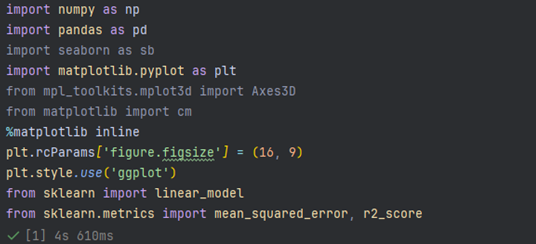
\includegraphics[width=1.0\textwidth]{Actividad-9/Imagen1.png}
    \caption{Importación de Librerias}
\end{figure}


El código comienza importando las bibliotecas esenciales para el análisis de datos y modelado estadístico. NumPy se utiliza para operaciones numéricas eficientes, mientras que Pandas permite manejar los datos en estructuras tabulares, facilitando su limpieza y exploración. Para la visualización, se carga Matplotlib junto con Seaborn, que mejoran la calidad estética de los gráficos. La línea \texttt{\%matplotlib inline} asegura que todas las visualizaciones se muestren directamente en el entorno de trabajo, ideal para Jupyter Notebook.

La configuración de \texttt{plt.rcParams} establece un tamaño predeterminado de 16x9 pulgadas para las figuras, lo que garantiza claridad al presentar los resultados. El estilo \texttt{'ggplot'} se aplica para dar a los gráficos un diseño más pulido, con colores atractivos y fondos grises que mejoran la legibilidad.

Finalmente, se importan las herramientas específicas para el modelado: \texttt{linear\_model} de Scikit-learn permite implementar la regresión lineal, mientras que \texttt{mean\_squared\_error} y \texttt{r2\_score} son métricas clave para evaluar el rendimiento del modelo. El MSE cuantifica el error promedio entre las predicciones y los valores reales, mientras que el R$^2$ indica qué porcentaje de la variabilidad en los datos logra explicar el modelo.

\subsection{Carga y exploración inicial de datos}

\begin{figure}[H]
    \centering
    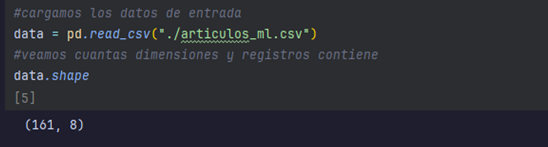
\includegraphics[width=1.0\textwidth]{Actividad-9/Imagen2.png}
    \caption{Carga de archivos}
\end{figure}

El código realiza la carga del conjunto de datos mediante la función \texttt{pd.read\_csv()}, que lee archivos en formato CSV y los convierte automáticamente en un DataFrame de Pandas, la estructura fundamental para trabajar con datos tabulares en Python. La ruta \texttt{"./articulos\_ml.csv"} indica que el archivo se encuentra en el mismo directorio donde se ejecuta el notebook. Es importante destacar que los DataFrames permiten manipular los datos de manera eficiente, ofreciendo operaciones para limpieza, filtrado y análisis.

Posteriormente, el comando \texttt{data.shape} muestra la dimensionalidad del DataFrame, devolviendo una tupla con dos valores: el primero (161) indica la cantidad de registros o filas, mientras que el segundo (8) representa el número de variables o columnas disponibles en el conjunto de datos. Esta salida es crucial para entender el alcance del análisis, confirmando que trabajaremos con 161 artículos diferentes, cada uno descrito por 8 características distintas.

\begin{figure}[H]
    \centering
    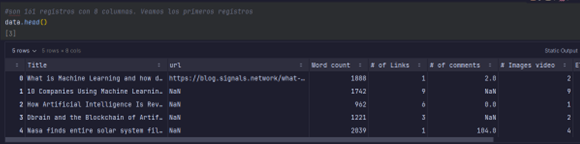
\includegraphics[width=1.0\textwidth]{Actividad-9/Imagen3.png}
    \caption{Primeras filas del dataset}
\end{figure}

El código \texttt{data.head()} es una herramienta fundamental para realizar una primera inspección de los datos cargados. Esta función muestra por defecto las primeras cinco filas del DataFrame, proporcionando una vista preliminar de la estructura y contenido del conjunto de datos. En este caso particular, podemos observar que efectivamente se visualizan 5 registros de los 161 existentes, cada uno con sus 8 columnas correspondientes.

\begin{figure}[H]
    \centering
    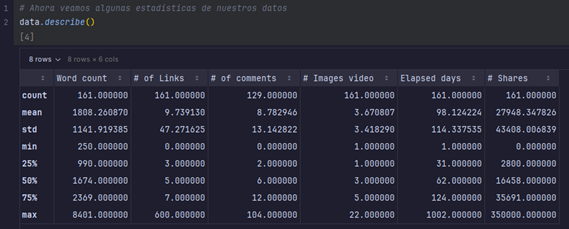
\includegraphics[width=1.0\textwidth]{Actividad-9/Imagen4.png}
    \caption{Estadísticas descriptivas del dataset}
    \label{fig:Carga y exploración inicial de datos}
\end{figure}

El comando \texttt{data.describe()} proporciona un resumen estadístico fundamental del conjunto de datos, ofreciendo una visión cuantitativa de la distribución de las variables numéricas. Esta función calcula automáticamente métricas clave para cada columna, permitiendo evaluar rápidamente el comportamiento de los datos.

Los resultados muestran estadísticas importantes para cada variable:
\begin{itemize}
    \item\textbf{Word count}: Los artículos tienen en promedio 1,808 palabras, con una gran variabilidad (desviación estándar de 1,141). El artículo más extenso contiene 8,401 palabras, mientras que el más breve solo 250.
    \item\textbf{\# Shares}: Variable objetivo del análisis, muestra una distribución asimétrica. El valor promedio es 27,948 compartidos, pero con una desviación estándar muy alta (43,408), indicando que algunos artículos son extremadamente virales comparados con la mayoría.
    \item\textbf{\# of Links}: Presenta una media de 9 enlaces por artículo.
\end{itemize}

Las diferencias entre medianas y medias en varias columnas (especialmente en "\# Shares" y "\# of comments") revelan distribuciones sesgadas, donde unos pocos artículos con valores extremadamente altos elevan el promedio general. Esto es particularmente evidente en el caso de los compartidos en redes sociales, donde el valor máximo (350,000) es casi diez veces mayor que el percentil 75 (35,691).

\subsection{Análisis de distribuciones mediante histogramas}

\begin{figure}[H]
    \centering
    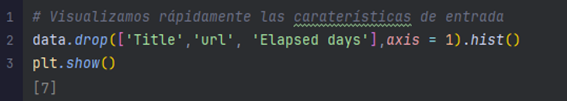
\includegraphics[width=1.0\textwidth]{Actividad-9/Imagen5.png}
    \caption{Visualizar histogramas}
\end{figure}

Tras haber examinado las estadísticas básicas con \texttt{describe()}, procedimos a visualizar las distribuciones de las variables numéricas. Para esto, ejecutamos la celda que genera los histogramas, eliminando primero las columnas no numéricas con \texttt{data.drop()} para enfocarnos en las variables relevantes.

\begin{figure}[H]
    \centering
    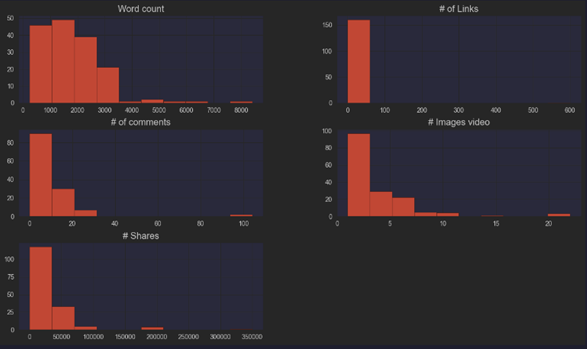
\includegraphics[width=1.0\textwidth]{Actividad-9/Imagen6.png}
    \caption{Histogramas de las variables numéricas}
\end{figure}

Los histogramas resultantes nos mostraron patrones clave en los datos. Observamos que la mayoría de artículos tenían entre 1,000 y 2,000 palabras, con algunos casos excepcionales más extensos. El número de compartidos presentó una distribución muy desigual, donde pocos artículos superaban ampliamente el promedio.

Esta visualización confirmó lo indicado por las estadísticas previas: la necesidad de procesar los valores extremos antes del modelado. Los gráficos también revelaron comportamientos interesantes en los comentarios y enlaces, mostrando concentraciones en valores específicos.

\subsection{Filtrado y visualización de datos}

\begin{figure}[H]
    \centering
    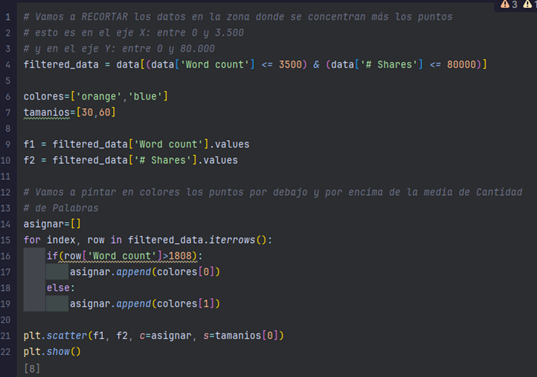
\includegraphics[width=1.0\textwidth]{Actividad-9/Imagen7.png}
    \caption{Visualzación de datos}
\end{figure}

Tras analizar las distribuciones, procedimos a limpiar el dataset eliminando valores extremos. El código aplica un filtro para conservar solo artículos con menos de 3,500 palabras y menos de 80,000 compartidos, lo que permite enfocarnos en la zona donde se concentra la mayoría de los datos. Este paso es crucial para mejorar la calidad del modelo, ya que reduce el efecto distorsionador de los outliers.

\begin{figure}[H]
    \centering
    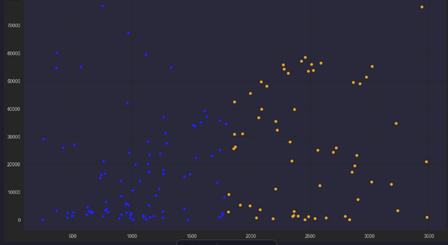
\includegraphics[width=1.0\textwidth]{Actividad-9/Imagen8.png}
    \caption{Relación entre palabras y compartidos}
\end{figure}

El gráfico de dispersión resultante muestra claramente la relación entre ambas variables. Los puntos se colorean según si superan (naranja) o no (azul) la media de palabras (1,808). Se observa que:

\begin{itemize}
    \item La mayoría de puntos se agrupan en la zona inferior izquierda
    \item Existe una ligera tendencia positiva: artículos más largos tienden a tener más compartidos
    \item La dispersión aumenta conforme crece el número de palabras
\end{itemize}

\subsection{Implementación del modelo de regresión lineal}

\begin{figure}[H]
    \centering
    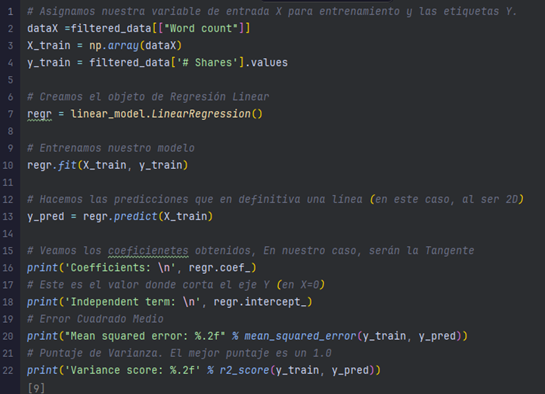
\includegraphics[width=1.0\textwidth]{Actividad-9/Imagen9.png}
    \caption{Construcción del modelo predictivo}
\end{figure}

Con los datos ya preparados, procedimos a construir el modelo predictivo. Primero asignamos las variables: utilizamos 'Word count' como variable independiente (X\_train) y '\# Shares' como variable objetivo (y\_train). Estas se convirtieron a arrays de NumPy para optimizar el procesamiento. El modelo se creó instanciando \texttt{LinearRegression()} y se entrenó con el método \texttt{fit()}.

\begin{figure}[H]
    \centering
    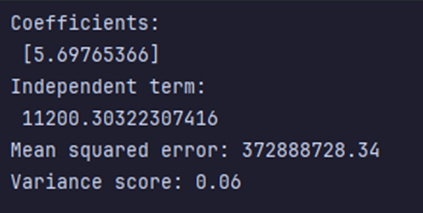
\includegraphics[width=1.0\textwidth]{Actividad-9/Imagen10.png}
    \caption{Resultados del modelo}
\end{figure}

Durante este proceso, el algoritmo calculó la relación óptima entre las palabras y los compartidos, generando una línea de mejor ajuste. Los resultados mostraron que:

\begin{itemize}
    \item Por cada palabra adicional, se predicen aproximadamente 5.70 compartidos más (coeficiente)
    \item El intercepto en 11,200 sugiere que incluso artículos muy breves tendrían esta base de compartidos
    \item El MSE de 372,888,728 indica un error considerable en las predicciones
    \item El R$^2$ de 0.06 revela que solo el 6\% de la variación en compartidos se explica por la longitud
\end{itemize}

Los valores obtenidos confirman lo observado en gráficos anteriores: existe una relación positiva pero débil entre ambas variables. El bajo score R$^2$ sugiere que la longitud del artículo por sí sola no es un predictor fuerte de viralidad, lo que indica la necesidad de incorporar variables adicionales en análisis futuros.

\section{Resultados}

\subsection{Visualización de los resultados del modelo}

\begin{figure}[H]
    \centering
    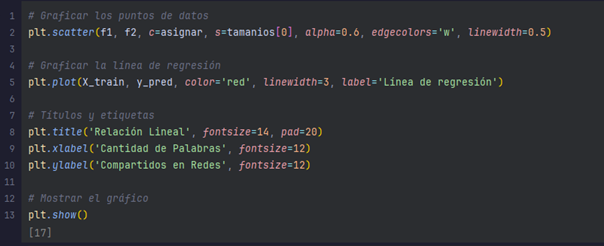
\includegraphics[width=1.0\textwidth]{Actividad-9/Imagen11.png}
    \caption{Generación del gráfico de regresión lineal}
\end{figure}

Para concluir el análisis, generamos un gráfico que combina los datos originales con la línea de regresión obtenida. El código utiliza \texttt{plt.scatter()} para mostrar los puntos filtrados anteriormente, manteniendo la codificación por colores (naranja para artículos sobre la media de palabras, azul para los demás). La transparencia (\texttt{alpha=0.6}) ayuda a visualizar mejor la densidad de puntos en zonas concurridas.

La línea de regresión se traza en rojo con \texttt{plt.plot()}, usando las predicciones del modelo (y\_pred) contra los valores reales de X\_train. Esta línea representa la relación lineal estimada: parte de aproximadamente 11,200 compartidos para artículos breves y tiene una pendiente suave de 5.7 compartidos por palabra adicional.

\begin{figure}[H]
    \centering
    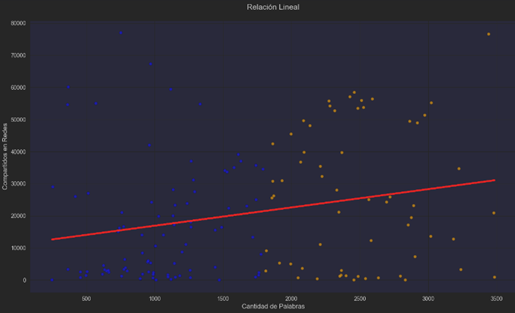
\includegraphics[width=1.0\textwidth]{Actividad-9/Imagen12.png}
    \caption{Modelo de regresión lineal superpuesto a los datos}
\end{figure}

\subsection{Hallazgos clave}
\begin{itemize}
    \item La línea confirma la relación positiva pero débil entre variables
    \item La dispersión de puntos alrededor de la línea explica el bajo R$^2$ (0.06)
    \item Se observan varios artículos "sobreperformers" (puntos naranjas altos) que superan ampliamente las predicciones
    \item La mayoría de artículos cortos (<1800 palabras) obtienen menos de 20,000 compartidos
\end{itemize}

El gráfico evidencia las limitaciones de usar solo la longitud del artículo como predictor. Si bien captura una tendencia general, la gran variabilidad residual sugiere que otros factores (calidad del contenido, tema, autor) influyen significativamente en el número de compartidos. Esto justifica el MSE elevado obtenido previamente.

\subsection{Predicción con el modelo entrenado}

\begin{figure}[H]
    \centering
    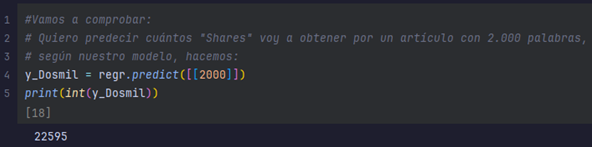
\includegraphics[width=1.0\textwidth]{Actividad-9/Imagen13.png}
    \caption{Validación del modelo}
\end{figure}

Para validar el modelo en un caso práctico, realizamos una predicción puntual de cuántos compartidos obtendría un artículo de 2,000 palabras. El código utiliza el método \texttt{predict()} sobre el modelo entrenado (\texttt{regr}), pasando como entrada el valor 2000 en un array bidimensional (formato requerido por scikit-learn).

El resultado obtenido fue 22,595 compartidos, lo que significa que:
\begin{itemize}
    \item Según el modelo, un artículo de esta longitud estaría ligeramente por encima del promedio observado
    \item La predicción sigue la tendencia lineal identificada (11,200 + 5.7*2000 = 22,600)
    \item Este valor debe interpretarse considerando el error cuadrático medio del modelo
\end{itemize}

\section{Conclusión}
El modelo de regresión lineal desarrollado identificó una relación estadísticamente significativa pero débil entre la longitud de los artículos y su desempeño en redes sociales. Si bien se confirmó que artículos más extensos tienden a recibir más compartidos (con un incremento promedio de 5.7 compartidos por palabra adicional), el bajo coeficiente de determinación (R$^2$ = 0.06) indica que la variable "Word count" explica solo una mínima parte de la variabilidad observada.

Los resultados obtenidos tienen importantes implicaciones prácticas:

\begin{itemize}
    \item \textbf{Para creadores de contenido}: Sugieren que aumentar la longitud de los artículos podría tener un efecto positivo marginal en su viralidad, pero que otros factores cualitativos (como el tema, calidad del contenido o autor) probablemente ejercen mayor influencia.
    
    \item \textbf{Para el modelo predictivo}: Evidencian la necesidad de incorporar variables adicionales que capturen dimensiones cualitativas del contenido, o explorar técnicas de modelado más sofisticadas que puedan manejar mejor la distribución asimétrica de los datos.
\end{itemize}

Las limitaciones principales encontradas fueron:
\begin{itemize}
    \item La presencia de valores atípicos extremos que afectan la estabilidad del modelo
    \item La distribución no lineal de los datos alrededor de la línea de regresión
    \item La gran variabilidad residual no explicada por la variable predictora
\end{itemize}

\end{document}